\documentclass[runningheads]{llncs}

%% Some recommended packages.
\usepackage{booktabs}   %% For formal tables:
                        %% http://ctan.org/pkg/booktabs
% \usepackage{subcaption} %% For complex figures with subfigures/subcaptions
                        %% http://ctan.org/pkg/subcaption
\usepackage{multirow}

\usepackage{listings}

\usepackage{graphicx}

\usepackage{subcaption}
\captionsetup{compatibility=false}

\usepackage{proof}

\usepackage{amsmath}

\usepackage{xcolor}

\usepackage{xspace}

\usepackage{wrapfig}

\usepackage{array}
\newcolumntype{e}[1]{>{\centering\let\newline\\\arraybackslash\hspace{0pt}}m{#1}}

\lstdefinelanguage{ocanren}{
keywords={run, conde, fresh, let, in, match, with, when, class, type,
object, method, of, rec, repeat, until, while, not, do, done, as, val, inherit,
new, module, sig, deriving, datatype, struct, if, then, else, open, private, virtual, include, success, failure,
true, false},
sensitive=true,
commentstyle=\small\itshape\ttfamily,
keywordstyle=\textbf,%\ttfamily\underline,
identifierstyle=\ttfamily,
basewidth={0.5em,0.5em},
columns=fixed,
mathescape=true,
fontadjust=true,
literate={fun}{{$\lambda$}}1 {->}{{$\to$}}3 {===}{{$\equiv$}}1 {=/=}{{$\not\equiv$}}1 {|>}{{$\triangleright$}}3 {\\/}{{$\vee$}}2 {/\\}{{$\wedge$}}2 {^}{{$\uparrow$}}1,
morecomment=[s]{(*}{*)}
}

\lstset{
%mathescape=true,
%basicstyle=\small,
%identifierstyle=\ttfamily,
%keywordstyle=\bfseries,
%commentstyle=\scriptsize\rmfamily,
%basewidth={0.5em,0.5em},
%fontadjust=true,
language=ocanren
}

\interfootnotelinepenalty=10000

\newcommand{\lstquot}[1]{``\lstinline{#1}''}
\newcommand{\sembr}[1]{\llbracket{#1}\rrbracket}
\newcommand{\false}{$f\!alse$}
\newcommand{\myif}{i\!f}
\newcommand{\mk}{\textsc{miniKanren}\xspace}
\newcommand{\muk}{\textsc{microKanren}\xspace}
\newcommand{\oc}{\textsc{OCanren}\xspace}
\newcommand{\ocaml}{\textsc{OCaml}\xspace}
\newcommand{\haskell}{\textsc{Haskell}\xspace}
\newcommand{\pro}{\textsc{Prolog}\xspace}
\newcommand{\scheme}{\textsc{Scheme}\xspace}
\newcommand{\todo}[1]{{\color{red}#1}}
\newcommand{\change}[1]{{\color{red}#1}}
\newcommand{\ecce}{\textsc{ECCE}\xspace}

\sloppy
% Used for displaying a sample figure. If possible, figure files should
% be included in EPS format.
%
% If you use the hyperref package, please uncomment the following line
% to display URLs in blue roman font according to Springer's eBook style:
% \renewcommand\UrlFont{\color{blue}\rmfamily}

\graphicspath{{figures/}}

\setlength{\textfloatsep}{5pt}
\setlength{\belowcaptionskip}{-3pt}
\setlength{\abovecaptionskip}{0pt}

\setlength{\abovedisplayskip}{-3pt}
\setlength{\belowdisplayskip}{-2pt}
\setlength{\abovedisplayshortskip}{0pt}
\setlength{\belowdisplayshortskip}{2pt}

\begin{document}

\title{An Empirical Study of Partial Deduction for \mk}

%
%\titlerunning{Abbreviated paper title}
% If the paper title is too long for the running head, you can set
% an abbreviated paper title here
%
\author{Anonymous author(s)}
%
\authorrunning{Anonymous author(s)}
% First names are abbreviated in the running head.
% If there are more than two authors, 'et al.' is used.
%
\institute{Anonymous institute(s)}


\maketitle

\begin{abstract}
  We study conjunctive partial deduction, an advanced specialization technique aimed at improving the performance of logic programs, in the context of relational programming language \mk. We identify a number of issues, caused by  \mk pecularities, and describe a novel approach to specialization based on partial deduction and supercompilation. While the results of the evaluation do not yet demonstrate the advantages of our approach in all cases, we nevertheless consider it as the first step towards an efficient optimization framework for \mk.
\end{abstract}


\section{Introduction}

A family of embedded domain-specific languages \mk\footnote{\mk language web site: \url{http://minikanren.org}} implement relational programming~---~a paradigm closely related to the pure logic programming.
The minimal core of the language, also known as \muk, can be implemented in as little as 39 lines of \scheme~\cite{friedmanmukanren}.
An introduction to the language and some of its extensions in a series of examples can be found in the book The Reasoned Schemer~\cite{TheReasonedSchemer}.
The formal certified semantics for \mk is described in~\cite{rozplokhas2020certified}.

Relational programming is a paradigm based on the idea of describing programs as relations.
The core feature of relational programming is the ability to run a program in various directions by executing goals with free variables.
The distribution of free variable occurrences determines the direction of relational search.
For example, having specified a relation for adding two numbers, one can also compute the subtraction of two numbers or find all pairs of numbers which can be summed up to get the given one.
One of the most prominent applications of relational programming amounts to implementing interpreters as relations.
By running a relational interpreter for some language \emph{backwards} one can do programs synthesis.
In general, it is possible to create a solver from a recognizer by translating it into \mk and running in the appropriate direction~\cite{lozov2019relational}.

The search employed in \mk is complete which means that every answer will be found, although it may take a long time.
The promise of \mk falls short when speaking of performance.
The execution time of a program in \mk is highly unpredictable and varies greatly for various directions.
What is even worse, it depends on the order of the relation calls within a program.
One order can be good for one direction, but slow down the computation dramatically in the other direction.

Partial evaluation~\cite{jonesbook} is a technique for specialization, i.e. improving the performance of a program given some information about it beforehand.
It may either be a known value of some argument, its structure (i.e. the length of an input list) or, in case of a relational program, --- the direction in which it is intended to be run.
An earlier paper~\cite{lozov2019relational} has shown that \emph{conjunctive partial deduction}~\cite{de1999conjunctive} can sometimes improve the performance of \mk programs.
Depending on the particular \emph{control} decisions, it may also not affect the execution time of a program or even make it slower.

Control issues in partial deduction of logic programming language \pro have been studied before~\cite{leuschel2002logic}.
Unlike Prolog, where atoms in the right-hand side of a clause cannot be arbitrarily reordered without changing the semantics of a program, in \mk the subgoals of conjunction/disjunction can be freely switched.
This opens yet another possibility for optimization, not taken into account by approaches initially developed in the context of conventional logic programming.
% The ideas described there make use of the deterministic search strategy of \pro.
% However in \mk it is allowed to reorder some relation calls within the goal for better performance.
% While sometimes conjunctive partial deduction gives great performance boost, sometimes it does not behave as well as it could have.

In this paper, we study issues which conjunctive partial deduction faces being applied for \mk.
We also describe a novel approach to partial deduction for relational programming, \emph{conservative partial deduction}.
We implemented this approach and compared it with the existing specialization system (\ecce) for several programs.
We report here the results of the comparison and discuss why some \mk programs run slower after specialization.

\section{Related Work}

Specialization is an attractive technique aimed to improve the performance of a program making use of its static properties such as known arguments or its environment.
Specialization is studied for functional, imperative, and logic programing and comes in different forms: partial evaluation~\cite{jonesbook} and partial deduction~\cite{lloyd1991partial}, supercompilation~\cite{soerensen1996positive}, distillation~\cite{hamilton2007distillation}, and many others.


The heart of supercompilation-based techniques is \emph{driving}~---~a symbolic execution of a program through all possible execution paths.
The result of driving is a possibly infinite \emph{process tree} where nodes correspond to \emph{configurations} which represent computation state.
For example, in the case of pure functional programming languages, the computational state might be a term.
Each path in the tree corresponds to some concrete program execution.
The two main sources for supercompilation optimizations are aggressive information propagation about variables' values, equalities and disequalities, and precomputing of deterministic semantic evaluation steps.
The latter process, also known as \emph{deforestation}~\cite{deforestation}, means  combining of consecutive process tree nodes with no branching.
When the tree is constructed, the resulting, or \emph{residual}, program can be extracted from the process tree by the process called \emph{residualization}.
Of course, the process tree can contain infinite branches.
\emph{Whistles} --- heuristics to identify possibly infinite branches --- are used to ensure supercompilation termination.
If a whistle signals during the construction of some branch, then something should be done to ensure termination.
The most common approaches are either to stop driving the infinite branch completely (no specialization is done in this case and the source code is blindly copied into the residual program) or to fold the process tree to a \emph{process graph}.
The main instrument to perform such a folding is some form of \emph{generalization}.
Generalization, abstracting away some computed data about the current term, makes folding possible.
%  i.e. abstracting away some computed data about the current term which makes folding possible.
One source of infinite branches is consecutive recursive calls to the same function with an accumulating parameter: by unfolding such a call further one can only increase the term size which leads to nontermination.
The accumulating parameter can be removed by replacing the call with its generalization.
There are several ways to ensure correctness and termination of a program transformer~\cite{sorensen1998convergence}, most-specific generalization
(anti-unification) and \emph{homeomorphic embedding}~\cite{Higman52,Kruskal60} as a
whistle being common.
%the most common being \emph{homeomorphic embedding}~\cite{Higman52,Kruskal60} used as a whistle and most-specific generalization of terms.
% When two dangerously similar nodes are encountered,
% For example, two consecutive recursive calls of a function with accumulating parameter, and the first is not an instance of the second, then one may construct a new, generalized, node such that both of original nodes are instances of the last one, then one of the initial nodes is replaced with the generalized one.

While supercompilation generally improves the behaviour of input programs and distillation can even provide superlinear speedup, there are no ways to predict the effect of specialization on a given program in general.
What is worse, the efficiency of a residual program from the target language evaluator point of view is rarely considered in the literature.
The main optimization source is computing in advance all possible intermediate and statically-known semantics steps at program transformation-time.
Other criteria, like the size of the generated program or possible optimizations and execution cost of different language constructions by the target language evaluator, are usually out of consideration~\cite{jonesbook}.
Partial evaluation in logic programming should be done with care to not interfere with the compiler optimizations~\cite{venken1988partial}.
It is also known that supercompilation may adversely affect GHC optimizations making standalone compilation more powerful~\cite{SCBE,TCES} and cause code explosion~\cite{SCHC}.
Moreover, it may be hard to predict the real speedup of any given program using concrete benchmarks even disregarding the problems above because of the complexity of the transformation algorithm.
The worst-case for partial evaluation is when all static variables are used in a dynamic context, and there is some advice on how to implement a partial evaluator as well as a target program so that specialization indeed improves its performance~\cite{jonesbook,bulyonkov84}.
There is a lack of research in determining the classes of programs which transformers would definitely speed~up.

Conjunctive partial deduction~\cite{de1999conjunctive} makes an effort to provide reasonable control for the left-to-right evaluation strategy of \pro.
CPD constructs a tree which models goal evaluation and is similar to an SLDNF tree, then a residual program is generated from the tree.
Partial deduction itself resembles driving in supercompilation~\cite{gluck1994partial}.
The specialization is done in two levels of control: the local control determines the shape of the residual programs, while the global control ensures that every relation which can be called in the residual program is defined.
The leaves of local control trees become nodes of the global control tree.
CPD analyses these nodes at the global level and runs local control for all those which are new.

At the local level, CPD examines a conjunction of atoms by considering each atom one-by-one from left to right.
An atom is \emph{unfolded} if it is deemed safe, i.e. a whistle based on homeomorphic embedding does not signal for the atom.
When an atom is unfolded, a clause whose head can be unified with the atom is found, and a new node is added into the tree where the atom in the conjunction is replaced with the body of that clause.
If there is more than one suitable head, then several branches are added into the tree which corresponds to the disjunction in the residualized program.
An adaptation of CPD for the \mk programming language is described in~\cite{lozov2019relational}.

\ecce partial deduction system~\cite{leuschel1997ecce} is the most mature implementation of CPD for \pro.
\ecce provides various implementations of both local and global control as well as several degrees of post-processing.
Unfortunately there is no automatic procedure to choose what control setting is likely to improve input programs the most.
The choice of the proper control is left to the user.

An empirical study has shown that the most well-behaved strategy of local control in CPD for \pro is \emph{deterministic unfolding}~\cite{leuschel1997advanced}.
An atom is unfolded only if precisely one suitable clause head exists for it with the one exception: it is allowed to unfold an atom non-deterministically once for one local control tree.
This means that if a non-deterministic atom is the leftmost one within a conjunction, it is most likely to be unfolded, introducing many new relation calls within the conjunction.
We believe this is the core problem of CPD which limits its power when applied to \mk.
The strategy of unfolding atoms from left to right is reasonable in the context of \pro because it mimics the way programs in \pro execute.
Special care should be taken when unfolding non-leftmost atoms in \pro: one should ensure that it does not duplicate code, as well as that no side-effects are done out of order~\cite{nonleftmost, leuschel2014fast}.
However in \mk leftmost unfolding often leads to larger global control trees and, as a result, bigger, less efficient programs.
On the contrary, according to the denotational semantics, the results of evaluation of a \mk program do not depend on the order of relation calls (atoms) within conjunctions, thus we believe a better result can be achieved by selecting a relation call which can restrict the number of branches in the tree.
We describe our approach, which implements this idea, in the next section.

\newcommand{\code}[1]{\texttt{#1}}

\section{Conservative Partial Deduction}

In this section, we describe a novel approach to relational programs specialization.
This approach draws inspiration from both conjunctive partial deduction and supercompilation.
The aim was to create a specialization algorithm which would be simpler than conjunctive partial deduction and use properties of \mk to improve the performance of the input programs.

The algorithm pseudocode is shown in Fig.~\ref{fig:ncpd-pseudo}.
For the sake of brevity and clarity, we provide functions \code{drive\_disj} and \code{drive\_conj} which describe how to process disjunctions and conjunctions respectively.
Driving itself is a trivial combination of the functions provided (line 2).

A driving process creates a process tree, from which a residual program is later created.
The process tree is meant to mimic the execution of the input program.
The nodes of the process tree include a \emph{configuration} which describes the state of program evaluation at some point.
In our case a configuration is a conjunction of relation calls.
The substitution computed at each step is also stored in the tree node, although it is not included in the configuration.

Hereafter, we consider all goals and relation bodies to be in \emph{canonical normal form}~---~a disjunction of conjunctions of either calls or unifications.
Moreover, we assume all fresh variables to be introduced into the scope and all unifications to be computed at each step.
Those disjuncts in which unifications fail are removed.
Each other disjunct takes the form of a possibly empty conjunction of relation calls accompanied with a substitution computed from unifications.
Any \mk term can be trivially transformed into the described form.
The function \code{normalize} in Fig.~\ref{fig:ncpd-pseudo} is assumed to perform term normalization.
The code is omitted for brevity.

\begin{figure}[!t]
  \centering
  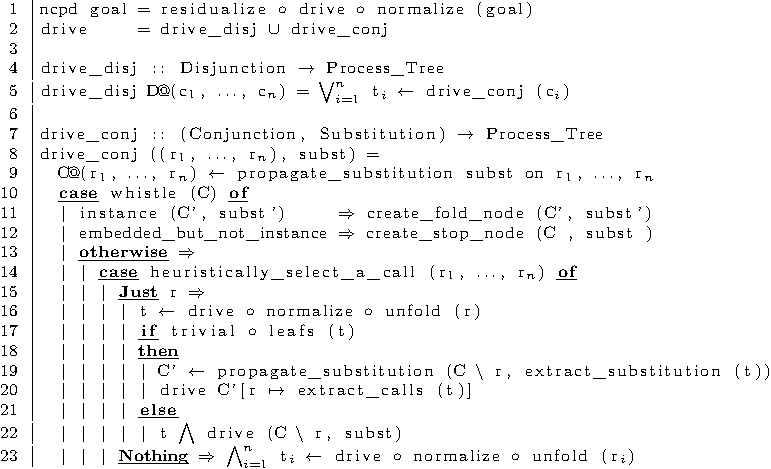
\includegraphics[width=\textwidth]{algo_pseudo-crop.pdf}
  \caption{Conservative partial deduction pseudo code}
  \label{fig:ncpd-pseudo}
\end{figure}

% The very first step of driving a conjunction is to apply a substitution to the variables in relation calls (line 10).

There are several core ideas behind this algorithm.
The first is to select an arbitrary relation to unfold, not necessarily the leftmost which is safe.
The second idea is to use a heuristics which decides if unfolding a relation call can lead to discovery of contradictions between conjuncts which in turn leads to restriction of the answer set at specialization-time (line 14; \code{heuristically\_select\_a\_call} stands for heuristics combination, see section~\ref{sec:heurictic} for details).
If those contradictions are found, then they are exposed by considering the conjunction as a whole and replacing the selected relation call with the result of its unfolding thus \emph{joining} the conjunction back together instead of using \emph{split} as in CPD (lines 15--22).
Joining instead of splitting is why we call our transformer \emph{conservative} partial deduction.
Finally, if the heuristics fails to select a potentially good call, then the conjunction is split into individual calls which are driven in isolation and are never joined (line 23).

When the heuristics selects a call to unfold (line 15), a process tree is constructed for the selected call \emph{in isolation} (line 16).
The leaves of the computed tree are examined.
If all leaves are either computed substitutions or are instances of some relations accompanied with non-empty substitutions, then the leaves are collected and each of them replaces the considered call in the root conjunction (lines 19--20).
If the selected call does not suit the criteria, the results of its unfolding are not propagated onto other relation calls within the conjunction, instead, the next suitable call is selected (line 22).
According to the denotational semantics of \mk it is safe to compute individual conjuncts in any order, thus it is ok to drive any call and then propagate its results onto the other calls.

% Each time we examine a conjunction of calls, we \emph{split} them into separate nodes which are driven independently from each other.
% Among the relation calls we select one which is according to the heuristic is likely to narrow down the answer set \db{(line 15)}.
% If the selected call does not suit the criteria, the results of its unfolding is not propagated onto other relation calls withing the conjunction and the next suitable call is selected \db{(line 22)}.

This process creates branchings whenever a disjunction is examined (lines 4--5).
At each step, we make sure that we do not start driving a conjunction which we have already examined.
To do this, we check if the current conjunction is a renaming of any other configuration in the tree (line 11).
If it is, then we fold the tree by creating a special node which then is residualized into a call to the corresponding relation.

In this approach, we do not generalize in the same fashion as CPD or supercompilation.
Our conjunctions are always split into individual calls and are joined back together only if it is meaningful.
If the need for generalization arises, i.e. homeomorphic embedding of conjunctions~\cite{de1999conjunctive} is detected, then we immediately stop driving this conjunction (line 12).
When residualizing such a conjunction, we just generate a conjunction of calls to the input program before specialization.

% The generalization is used in supercompilation and partial deduction to ensure termination at the same time as some degree of specialization.
% The generalization of two terms is usually a \emph{most-specific generalization}.
% Generalization is used to abstract away some information computed during driving.
% In conjunctive partial deduction generalization is modified to support treating of conjunctions.
% The generalization selects subconjuctions of two conjuncts which are similar (call to the same relation and their arguments have similar shape and distribution).
% For the subconjunctions selected a most-specific generalization is computed.

% In our approach we only do splitting of a conjunction into individual relation calls.
% This makes any program with an accumulating parameter to be a problem.
% Sometimes when there is a need to do a proper generalization, it is in reality just an instance of some other goal within the tree and we can simply create a call there \db{(line 13)}.
% Otherwise we are unable to meaningfully specialize such goal, but we can always just include the initial program in the residual program and call the corresponding relation.


\subsection{Unfolding}

Unfolding in our case is done by substitution of some relation call by its body with simultaneous normalization and computation of unifications.
% To unfold a relation call we do the following steps.
% \db{TODO: the following has alredy mentioned above.}
% First, the formal arguments of a relation are substituted for the actual arguments of the call in the body.
% All fresh variables get instantiated.
% The body is transformed into a canonical form (disjunction of conjunctions of either calls or unifications).
% All unifications are computed.
% Those disjuncts in which unifications fails are removed.
% Other disjuncts take form of a conjunction of relation calls accompanied with a substitution.
The unfolding itself is straightforward; however it is not always clear what to unfold and when to \emph{stop} unfolding.
Unfolding in the context of specialization of functional programming languages, as well as inlining in specialization of imperative languages, is usually considered to be safe from the residual program efficiency point of view.
It may only lead to code explosion or code duplication which is mostly left to a target program compiler optimization or even is out of consideration at all if a specializer is considered as a standalone tool~\cite{jonesbook}.

Unfortunately, this is not the case for the specialization of a relational programming language.
Unlike functional and imperative languages, in logic and relational programming languages unfolding may easily affect the target program's efficiency~\cite{leuschel2002logic}.
Unfolding too much may create extra unifications, which is by itself a costly operation, or even introduce duplicated computations by propagating the results of unfolding onto neighbouring conjuncts.

There is a fine edge between too much unfolding and not enough unfolding.
The former is maybe even worse than the latter.
We believe that the following heuristics provides a reasonable approach to unfolding control.

\subsection{Less Branching Heuristics}
\label{sec:heurictic}

This heuristics is aimed at selecting a relation call within a conjunction which is both safe to unfold and may lead to discovering contradictions within the conjunction.
An unsafe unfolding leads to an uncontrollable increase of the number of relation calls in a conjunction.
It is best to first unfold those relation calls which can be fully computed up to substitutions.

We deem every static (non-recursive) conjunct to be safe because they never lead to growth in the number of conjunctions.
Those calls which unfold deterministically, meaning there is only one disjunct in the unfolded relation, are also considered to be safe.

Those relation calls which are neither static nor deterministic are examined with what we call the \emph{less-branching} heuristics.
It identifies the case when the unfolded relation contains fewer disjuncts than it could possibly have.
This means that we found some contradiction, some computations were gotten rid of, and thus the answer set was restricted, which is desirable when unfolding.
To compute this heuristics we precompute the maximum possible number of disjuncts in each relation and compare this number with the number of disjuncts when unfolding a concrete relation call.
The maximum number of disjuncts is computed by unfolding the body of the relation in which all relation calls were replaced by a unification which always succeeds.

\begin{figure}[!t]
  \centering
  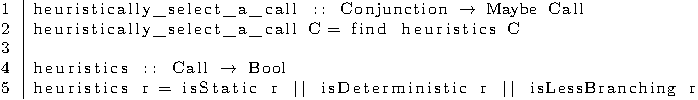
\includegraphics[width=\textwidth]{heuristic-crop.pdf}
  \caption{Heuristics selection pseudocode}
  \label{fig:heu-pseudo}
\end{figure}

%  more complicated case is when there are less disjuncts than there can possibly be.
% This signifies that at least one branch of computations is gotten rid of.

The pseudocode describing our heuristics is shown in Fig.~\ref{fig:heu-pseudo}.
Selecting a good relation call can fail (line 1).
The implementation works such that we first select those relation calls which are static, and only if there are none, we proceed to consider deterministic unfoldings and then we search for those which are less branching.
We believe this heuristics provides a good balance in unfolding.
% The final heuristic selects the first conjunct which suites either of the following cases.
% First we unfold those conjuncts which are static.
% Then --- deterministic.
% Then those which are less branching.
% The last to be unfolded are those calls, which unfold to a substitution with not conjunction.

% \subsection{Residualization}

% Residualization is quite straightforward.
% A branching in the process tree becomes a disjunction.
% A split node becomes a conjunction.
% Computed substitution is residualized as a conjunction of unifications.
% A renaming node is just a call to a relation.
% Relations are created for configurations on which leaf nodes are renamed.

% One other thing is that when some configuration is occurred within the tree which is an instance of a configuration for which a new relation is created, then we just create a call.

\section{Evaluation}

We implemented the conservative partial deduction for \mk and compared it with the \ecce partial deduction system.
\ecce is designed for \pro programming language and cannot be directly applied for programs, written in \mk.
To be able to compare our approach with \ecce, we converted each input program first to the pure subset of \pro, then specialized it with \ecce, and then we converted the result back to \mk.
The conversion to \pro is a simple syntactic conversion. In the conversion from \pro to \mk, for each Horn clause a conjunction is generated in which unifications are placed before any relation call.

We chose two problems for our study: evaluation of a subset of propositional formulas and typechecking for a simple language.
The problems illustrate the approach of using relational interpreters to solve search problems~\cite{lozov2019relational}.
For both these problems we considered several possible implementations in \mk which highlight different aspects relevant in specialization.

The \lstinline{eval$^o$} relation implements an evaluator of a subset of propositional formulas.
We consider four different implementations of this relation to explore how the way program is implemented can affect the quality of specialization.
Depending on the implementation, \ecce generates programs of varying performance, while the execution times of the programs generated by our approach are similar.

The \lstinline{typecheck$^o$} relation implements a typechecker for a tiny expression language.
We consider two different implementations of this relation: one written by hand and the other generated from the functional program.
We demonstrate how much these implementations differ in terms of performance before and after specialization.

In this study we measured the execution time for the sample queries, averaging them over multiple runs.
We also measured the number of unifications done in search of each individual answer.
All examples of \mk relations in this paper are written in \oc\footnote{\oc: statically typed \mk embedding in \ocaml. The repository of the project: \url{https://github.com/JetBrains-Research/OCanren}}.
The queries were run on a laptop running Ubuntu 18.04 with quad core Intel Core i5 2.30GHz CPU and 8 GB of RAM.

The tables and graphs use the following denotations.
\emph{Original} represents the execution time of a program before any transformations were applied; \emph{ECCE}~--- of the program specialized by \ecce with default conjunctive control setting; \emph{ConsPD}~--- of the program specialized by our approach.

\subsection{Evaluator of Logic Formulas}

The relation \lstinline{eval$^o$} describes an evaluation of a propositional formula under given variable assignments.
The relation has three arguments. The first argument is a list of boolean values which plays a role of variable assignments.
The $i$-th value of the substitution is the value of the $i$-th variable.
The second argument is a formula with the following abstract syntax.
A formula is either a \emph{variable} represented with a Peano number, a \emph{negation} of a formula, a \emph{conjunction} of two formulas or a \emph{disjunction} of two formulas.
The third argument is the value of the formula under the given assignment.

We specialize the \lstinline{eval$^o$} relation to synthesize formulas which evaluate to \lstinline{^true}.
To do so, we run the specializer for the goal with the last argument fixed to \lstinline{^true}, while the first two arguments remain free variables.
Depending on the way the \lstinline{eval$^o$} is implemented, different specializers generate significantly different residual programs.

\subsubsection{The Order of Relation Calls}

One possible implementation of the evaluator is presented in Listing~\ref{eval:last}.
Here relation \lstinline{elem$^o$ subst v res} unifies \lstinline{res} with the value of the variable \lstinline{v} in the list \lstinline{subst}.
The relations \lstinline{and$^o$}, \lstinline{or$^o$}, and \lstinline{not$^o$} encode corresponding boolean connectives.

\begin{figure*}[!t]
  \centering
  \begin{minipage}{0.95\textwidth}
    \begin{lstlisting}[label={eval:last}, caption={Evaluator of formulas with boolean operation last}, captionpos=b, frame=tb]
  let rec eval$^o$ subst fm res = conde [fresh (x y z v w) (
      (fm === conj x y /\ eval$^o$ st x v /\  eval$^o$ st y w /\  and$^o$ v w res);
      (fm === disj x y /\ eval$^o$ st x v /\  eval$^o$ st y w /\  or$^o$   v w res);
      (fm === neg x    /\ eval$^o$ st x v /\  not$^o$ v res));
      (fm === var v    /\ elem$^o$ subst v res)]
    \end{lstlisting}
  \end{minipage}
  \begin{minipage}{0.95\textwidth}
    \begin{lstlisting}[label={eval:fst}, caption={Evaluator of formulas with boolean operation second}, captionpos=b, frame=tb]
  let rec eval$^o$ subst fm res = conde [fresh (x y z v w) (
      (fm === conj x y /\ and$^o$ v w res /\  eval$^o$ st x v /\  eval$^o$ st y w);
      (fm === disj x y /\ or$^o$   v w res /\ eval$^o$ st x v /\  eval$^o$ st y w);
      (fm === neg x    /\ not$^o$ v res   /\ eval$^o$ st x v);
      (fm === var v    /\ elem$^o$ subst v res))]
    \end{lstlisting}
  \end{minipage}
\end{figure*}

Note, the calls to boolean relations \lstinline{and$^o$}, \lstinline{or$^o$}, and \lstinline{not$^o$} are placed last within each conjunction.
This poses a challenge for the CPD-based specializers such as \ecce.
Conjunctive partial deduction unfolds relation calls from left to right, so when specializing this relation for running backwards (i.e. considering the goal \lstinline{eval$^o$ subst fm ^true}), it fails to propagate the direction data onto recursive calls of \lstinline{eval$^o$}.
Knowing that \lstinline{res} is \lstinline{^true}, we can conclude that in the call \lstinline{and$^o$ v w res} variables \lstinline{v} and \lstinline{w} have to be \lstinline{^true} as well.
There are three possible options for these variables in the call \lstinline{or$^o$ v w res} and one for the call \lstinline{not$^o$}.
These variables are used in recursive calls of \lstinline{eval$^o$} and thus restrict the result of driving.
CPD fails to recognize this, and thus unfolds recursive calls of \lstinline{eval$^o$} applied to fresh variables.
It leads to over-unfolding, large residual programs and poor performance.

The conservative partial deduction first unfolds those calls which are selected according to the heuristics.
Since exploring the implementations of boolean connectives makes more sense, they are unfolded before recursive calls of \lstinline{eval$^o$}.
The way conservative partial deduction treats this program is the same as it treats the other implementation in which boolean connectives
are moved to the left, as shown in Listing~\ref{eval:fst}.
This program is easier for \ecce to specialize which demonstrates how unequal the behaviour of CPD for similar programs is.

\subsubsection{Unfolding of Complex Relations}

Depending on the way a relation is implemented, it may take a different number of driving steps to reach the point when any useful information is derived through its unfolding.
Partial deduction tries to unfold every relation call unless it is unsafe, but not all relation calls serve to restrict the search space and thus should be unfolded.
In the implementation of \lstinline{eval$^o$} boolean connectives can effectively restrict variables within the conjunctions and should be unfolded until they do.
But depending on the way they are implemented, the different number of driving steps should be performed for that.
The simplest way to implement these relations is by mimicking a truth tables as demonstrated by the implementation of \lstinline{not$^o$} in Listing~\ref{not:table}.
It is enough to unfold such relation calls once to derive useful information about variables.

\begin{figure*}[!t]
  \centering
  \begin{minipage}{0.5\textwidth}
    \begin{lstlisting}[label={not:table}, caption={Implementation of boolean \lstinline{not} as a table}, captionpos=b, frame=tb]
  let not$^o$ x y = conde [
     (x === ^true /\ y === ^false;
      x === ^false /\ y === ^true)]
    \end{lstlisting}
  \end{minipage}
  \begin{minipage}{0.8\textwidth}
    \begin{lstlisting}[label={not:nando}, caption={Implementation of boolean operation via \lstinline{nand}}, captionpos=b, frame=tb]
  let not$^o$   x y = nand$^o$ x x y
  let or$^o$   x y z = nand$^o$ x x xx /\  nand$^o$ y y yy /\ nand$^o$ xx yy z
  let and$^o$ x y z = nand$^o$ x y xy /\   nand$^o$ xy xy z
  let nand$^o$ a b c = conde [
    ( a === ^false /\ b === ^false /\ c === ^true );
    ( a === ^false /\ b === ^true  /\ c === ^true );
    ( a === ^true  /\ b === ^false /\ c === ^true );
    ( a === ^true  /\ b === ^true  /\ c === ^false)]
    \end{lstlisting}
  \end{minipage}
\end{figure*}

The other way to implement boolean connectives is to express them using a single basic boolean relation such as \lstinline{nand$^o$} which is, in turn, has a table-based
implementation (see Listing~\ref{not:nando}). It will take several sequential unfoldings to derive that variables \lstinline{v} and \lstinline{w} should
be \lstinline{^true} when considering a call \lstinline{and$^o$ v w ^true} implemented via a basic relation.
Conservative partial deduction drives the selected call until it derives useful substitutions for the variables involved while CPD with deterministic unfolding may fail to do so.


\subsubsection{Evaluation Results}

In our study we considered 4 implementations of \lstinline{eval$^o$} summed up in the table~\ref{tbl:eval}. They differ in the way the boolean connectives are implemented (see column \emph{Implementation}) and whether they are placed before or after the recursive calls to \lstinline{eval$^o$} (see column \emph{Placement}).
These four implementations are very different from the  standpoint of \ecce.

\begin{table}[!h]
    \centering
    \begin{tabular}{c||c||c}
                      & Implementation & Placement \\ \hline\hline
    \emph{FirstPlain} & table-based    & before \\ \hline
    \emph{LastPlain}  & table-based    & after  \\ \hline
    \emph{FirstNando} & via nand$^o$   & before \\ \hline
    \emph{LastNando}  & via nand$^o$   & after  \\
    \end{tabular}

  \caption{Different implementations of eval$^o$}
  \label{tbl:eval}
\end{table}

We measured the time necessary to generate $1000$ formulas over two variables which evaluate to \lstinline{^true} (averaged over 10 runs).
The results are presented in Fig.~\ref{fig:eval}.

\begin{figure}[!t]
  \centering
  \begin{subfigure}[c]{0.35\textwidth}
    \centering
    \begin{tabular}{e{1cm}||c|c|c}
               & Original & \ecce & ConsPD \\ \hline\hline
      \emph{FirstPlain} & 1.59s & 1.61s & 0.92s \\ \hline
      \emph{FirstNando} & 1.43s & 2.24s & 0.96s \\ \hline
      \emph{LastPlain}  & 0.98s & 1.43s & 0.97s \\ \hline
      \emph{LastNando}  & 1.09s & 1.54s & 0.91s
    \end{tabular}
  \end{subfigure}
  \hfill
  \begin{subfigure}[c]{0.58\textwidth}
    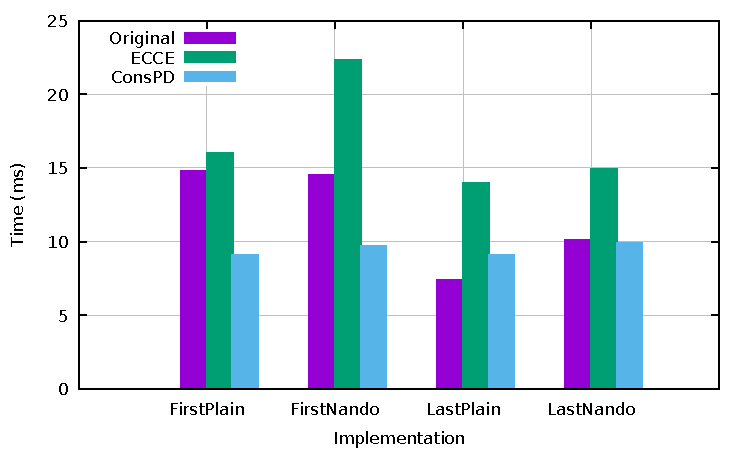
\includegraphics[width=\textwidth]{data/propEval/prop.pdf}
  \end{subfigure}
  \caption{Execution time of evalo}
  \label{fig:eval}
\end{figure}

Conservative partial deduction generates  programs with comparable performance for all four implementations, while the quality of \ecce specialization differs significantly.
\ecce worsens performance for every implementation as compared to the original program.
ConsPD do not worsen performance for any implementation.
Its effect is most significant for the implementations in which the boolean connectives are placed first within conjunctions.

\subsubsection{The Order of Answers}

It is important to note that different implementations of the same \mk relation produce answers in different orders.
Nevertheless, since \mk search is complete, all answers will be found eventually.
Unfortunately, it is not guaranteed that the first 1000 formulas generated with different implementations of \lstinline{eval$^o$} will be the same.
For example, $983$ formulas are the same among the first $1000$ formulas generated by the Original \emph{FirstPlain} relation and the same relation after the ConsPD transformation.
At the same time, only $405$ formulas are the same between the Original and \ecce \emph{LastNando} relations.

The reason why implementations differ so much in the order of the answers stems from the canonical search strategy employed in \mk.
Most \mk implementations employ \emph{interleaving} search~\cite{10.1145/1090189.1086390} which is left-biased.
It means that the leftmost disjunct in a relation is being executed longer than the disjunct on the right.
This property is not local which makes it very hard to estimate the performance of a given relation.

In practice it means that if a specializer reorders disjuncts, then the performance of relations after specialization may be unpredictable.
For example, by putting the disjuncts of the \lstinline{eval$^o$} relation in the opposite order, one produces a relation which runs much faster than the original, but it generates completely different formulas at the same time.
Most of the first 1000 formulas in this case are multiple negations of a variable, while the original relation produces more diverse set of answers.
Computing a negation of a formula only takes one recursive \lstinline{eval$^o$} call thus finding such answers is faster than conjunctions and disjunctions.
Meanwhile, the formulas generated by the reordered relation are less diverse and may be of less interest.

Although neither \ecce nor ConsPD reorder disjuncts, they remove disjuncts which cannot succeed.
Thus they influence the order of answers and performance of relations.
We believe that, in general, it is not possible to guarantee the same order of answers after specialization.
Exploring how different specializations influence the execution order is a fascinating direction for future research.


\subsection{Typechecker-Term Generator}

This relation implements a typechecker for a tiny expression language.
Being executed in the backward direction it serves as a generator of terms of the given type.
The abstract syntax of the language is presented below.
The variables are represented with de Bruijn indices, thus let-binding does not specify which variable is being bound.

\[\begin{array}{lllll}
  type \ term = &\ BConst \ of \ Bool &| \ IConst \ of \ Int &| \ Var \ of \ Int & \\
  & | \ term + term &| \ term * term &| \ term = term &| \ term < term \\
  &| \ \underline{let} \ term \ \underline{in} \ term
  &\multicolumn{2}{l}{| \ \underline{if} \ term \ \underline{then} \ term \ \underline{else} \ term} &
\end{array}\]

The typing rules are straightforward and are presented below.
Boolean and integer constants have the corresponding types regardless of the environment.
Only terms of type integer can be summed up, multiplied or compared by less-than operator.
Any terms of the same type can be checked for equality.
Addition and multiplication of two terms of suitable types have integer type, while comparisons have boolean type.
If-then-else expression typechecks only if its condition is of type boolean, while both then- and else-branches have the same type.
An environment $\Gamma$ is an ordered list, in which the $i$-th element is the type of the variable with the $i$-th de Bruijn index.
To typecheck a let-binding, first, the term being bound is typechecked and is added in the beginning of the environment $\Gamma$, and then the body is typechecked in the context of the new environment.
Typechecking a variable with the index $i$ boils down to getting an $i$-th element of the list.

\begin{table}[!h]
  \setlength{\tabcolsep}{0.4cm}
  \centering
  \begin{tabular}{c c c}
    \infer[]{\Gamma \vdash IConst \ i : Int}{} &
    \infer[]{\Gamma \vdash BConst \ b : Bool}{}  &
    \infer[\Gamma \lbrack v \rbrack \equiv \tau]{\Gamma \vdash Var \ v : \tau}{} \vspace{0.5cm}
    \\
    \infer[]{\Gamma \vdash t + s : Int}{\Gamma \vdash t : Int, \Gamma \vdash  s : Int}  \vspace{0.5cm} &
    \infer[]{\Gamma \vdash t = s : Bool}{\Gamma \vdash t : \tau, \Gamma \vdash  s : \tau} &
    \infer[]{\Gamma \vdash \underline{let} \ v \ b : \tau}{\Gamma \vdash v : \tau_v, \ (\tau_v :: \Gamma) \vdash b : \tau}
      \\

      \infer[]{\Gamma \vdash t * s : Int}{\Gamma \vdash t : Int, \Gamma \vdash  s : Int}  &
    \infer[]{\Gamma \vdash t < s : Bool}{\Gamma \vdash t : Int, \Gamma \vdash  s : Int} \vspace{0.5cm} &
      \infer[]{\Gamma \vdash \underline{if} \ c \ \underline{then} \ t \ \underline{else} \ s : \tau}{\Gamma \vdash c : Bool, \Gamma \vdash t : \tau, \Gamma \vdash s : \tau}
  \end{tabular}
\end{table}


We compared two implementations of these typing rules.
The first one is obtained by unnesting of a functional program as described in~\cite{lozov2019relational} (\emph{Generated}).
It is worth noting that the unnesting introduces a lot of redundancy in form of extra unifications and thus creates programs which are very inefficient.
Thus we contrast this implementation with the program hand-written in \oc (\emph{Hand-written}).
Each implementation has been specialized with ConsPD and \ecce.
We measured the time needed to generate 1000 closed terms of type integer (see Fig.~\ref{tbl:type}).


\begin{figure}[!h]
  \begin{subfigure}[c]{0.55\textwidth}
    \centering
    \begin{tabular}{c||c|c|c}
                          & Original & \ecce & ConsPD  \\ \hline\hline
      \emph{Hand-written} & 0.92s    & 0.22s & 0.34s   \\ \hline
      \emph{Generated}    & 11.46s   & 0.38s & 0.29s
      \end{tabular}
  \end{subfigure}
  \hfill
  \begin{subfigure}[c]{0.45\textwidth}
    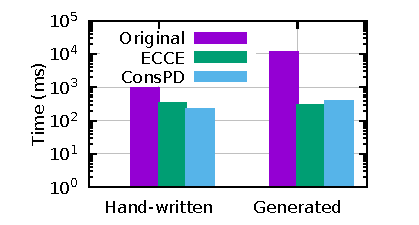
\includegraphics[width=\textwidth]{data/lTypecheck/ltypelog.pdf}
  \end{subfigure}
  \caption{Execution  time of generating 1000 closed terms of type Integer}
  \label{tbl:type}
\end{figure}

As expected, the generated program is far slower than the hand-written.
The principal difference between these two implementations is that the generated program contains a certain redundancy introduced by unnesting.
For example, typechecking of the sum of two terms in the hand-written implementation consists of a single conjunction (see Listing~\ref{type:hand}) while the generated program is far more complicated and also uses a special relation \lstinline{typeEq$^o$} to compare types (see Listing~\ref{type:gen}).

\begin{figure*}[!h]
  \centering
    \begin{lstlisting}[label={type:hand}, caption={A fragment of hand-written typechecker}, captionpos=b, frame=tb]
  let rec typecheck$^o$ gamma term res = conde [
    ...
    fresh (x y) ((term === x + y /\
       typecheck$^o$ gamma x ^(Some Integer) /\
       typecheck$^o$ gamma y ^(Some Integer) /\
       res === ^(Some Integer)));
    ...]
    \end{lstlisting}
\end{figure*}


\begin{figure*}[!t]
  \centering
    \begin{lstlisting}[label={type:gen}, caption={A fragment of generated typechecker}, captionpos=b, frame=tb]
let rec typecheck$^o$ gamma term res = conde [
  ...
  fresh (x y t1 t2) ((term === x + y /\
    conde [
      typecheck$^o$ gamma x ^None       /\ res === ^None;
      typecheck$^o$ gamma x ^(Some t1) /\
        typecheck$^o$ gamma y ^None     /\ res === ^None;
      typecheck$^o$ gamma x ^(Some t1) /\  typecheck$^o$ gamma y ^(Some t2) /\
        typeEq$^o$ t1 Integer ^true     /\ typeEq$^o$ t2 Integer ^true /\
        res === ^(Some Integer);
    ])
  ...]
    \end{lstlisting}
\end{figure*}

Most of the redundancy of the generated program is removed by specialization with respect to the known type of the term.
This is why both implementations have comparable speed after specialization.
\ecce shows bigger speedup for the hand-written program than ConsPD and vice versa for the generated implementation.
We believe that this difference can be explained by too much unfolding.
\ecce performs a lot of excessive unfolding for the generated program and only barely changes the hand-written program.
At the same time ConsPD specializes both implementations to comparable programs performing average amount of unfolding.
This shows that the heuristics we presented gives more stable, although not the best, results.

% У заключения нет номера главы
\clearpage

\section*{Заключение}
В ходе данной работы получены следующие результаты. 
\begin{itemize}
  \item Изучена предметная область: методы обработки встроенных языков и алгоритм обобщённого синтаксического анализа RNGLR.
  \item Разработан алгоритм синтаксического анализа динамически формируемых выражений, поддерживающий работу с произвольными входными графами.
  \item Доказана корректность алгоритма:
  \begin{itemize}
    \item алгоритм завершит работу для любых входных данных;
          %для любой входной детерминированной контекстно-свободной грамматики и 
          %произвольного входного графа алгоритм завершит свою работу;
    \item для любой цепочки из входного множества, выводимой в эталонной грамматике G, в SPPF содержится её дерево вывода в G; при этом никакие другие деревья не содержатся в SPPF.
          %для любой цепочки, которую может породить автомат (которая содержится 
          %в регулярном множестве), выводимой в рассматриваемой грамматике G, в 
          %SPPF содержится её дерево вывода в G, при этом не содержится никаких 
          %других деревьев.
  \end{itemize}
  \item Выполнена реализация алгоритма на языке программирования F\# в рамках исследовательского проекта YaccConstructor.
  \item Проведена апробация: регрессионное тестирование, тестирование производительности и тестирование на реальных данных.
  \item Исходный код проекта YaccConstructor можно найти на сайте \url{https://github.com/YaccConstructor/YaccConstructor}, автор принимал участие под учётной записью kajigor.
\end{itemize}

В дальнейшем планируется изменить алгоритм таким образом, чтобы помимо 
построения леса разбора всех корректных выражений осуществлялся бы также поиск ошибочных выражений и сообщение о них. Также необходимо произвести теоретическую оценку сложности алгоритма. Предложенный алгоритм планируется внедрить в инструмент по реинжинирингу информационных систем.  

\bibliographystyle{splncs04.bst}
\bibliography{bibl.bib}

\end{document}
